\documentclass[12pt]{article}
\usepackage{fancyhdr}
\usepackage{lastpage}
\usepackage{geometry}
\usepackage{amsmath}
\usepackage{setspace}
\usepackage{graphicx}
\usepackage{caption}
\geometry{a4paper,scale=0.8}
\pagestyle{plain}
\renewcommand{\headrulewidth}{0.4pt}
\renewcommand{\footrulewidth}{0.4pt}
\setlength{\baselineskip}{23pt}


\begin{document}
	\thispagestyle{plain}

\section{SMB, HML and UMD: A Deeper Dive}


\noindent While our findings are generally in line with and supportive of the three-factor model first introduced by Fama and French (1993), a point of divergence arises from our observed mean values of SMB and HML over our sample period. We observed mean values of -0.59\% (mildly statistically significant at 95\% confidence) and -0.35\% (statistically insignificant at 95\% confidence) for our SMB and HML values respectively, which comes in contrast to Fama and French's (1993) observed mean values of 0.27\% and 0.40\%, especially with regards to the signs of the means. Our observed mean $R_m - R_f$ factor is in line with the one observed in original Fama and French (1993) study. We also look into an additional factor, Up Minus Down (UMD), a proxy for stock return momentum, in this section.\\

\noindent To further examine the behaviour of the SMB, HML and UMD factors over time and how the mean factor realisations can possibly diverge, we treated the factor realisations as actual portfolio returns and tracked the cumulative returns of the constructed portfolios over time. \\

\noindent For this purpose, we utilised monthly Fama-French Factors data between January 1929 to December 2018 provided by WRDS and plotted the cumulative returns of the respective portfolio over this extended sample period. Also, given how monthly SMB, HML and UMD factor realisations tend to have a high level of noise from month to month, we used 7-year rolling averages of the SMB, HML and UMD readings as a gauge of the changes in the broader trends of the respective time series.\\

\noindent \textbf{The SMB Factor}

\noindent For the SMB factor, we found that the factor realisations do not exhibit consistently positive readings over our sample period, though said SMB readings are, on average, mildly positive (at 0.21\%). When using the SMB factor as a proxy, we also observed that the small-firm effect highlighted by Banz (1981) quickly dissipated and even reversed in the years following the publication of his findings, though these two events may have had happened by mere coincidence.

\begin{figure}[h]
	\centering
	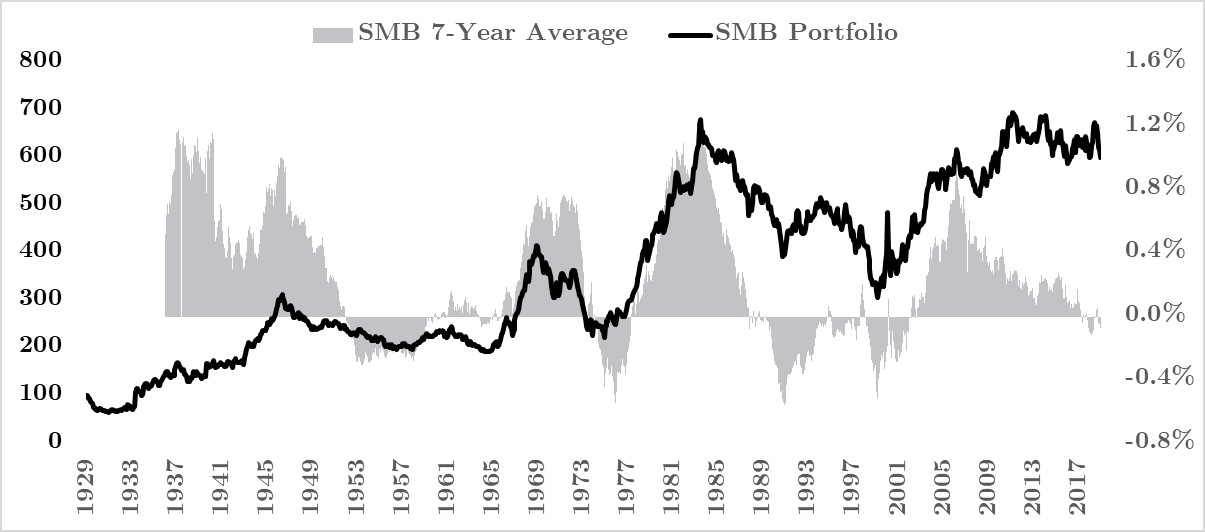
\includegraphics[width=0.9\linewidth]{SMB01}
	\caption*{Fig 01: SMB Portfolio \& Rolling 7-Year Average SMB Returns}
	\label{fig:label}
\end{figure}

\noindent The rolling 7-year SMB average plotted in Fig 01 (grey column chart) shows how the SMB factor realisations have trended in and out of positive territories over our extended sample period. The fluctuations in the level of our constructed SMB Portfolio (blue line chart in Fig 01, starting portfolio size = 100) also highlight the earlier-mentioned point, though the net gain the portfolio has clocked over the extended sample period suggests that SMB factor realisations are still on average, positive. The sample period used in our main study (July 2011 - December 2018) happens to denote a time period when rolling 7-year average SMB factor realisations have once again flipped over to the negative regions, thus explaining the divergence between our observed mean SMB and that of Fama and French (1993).

\begin{figure}[h]
	\centering
	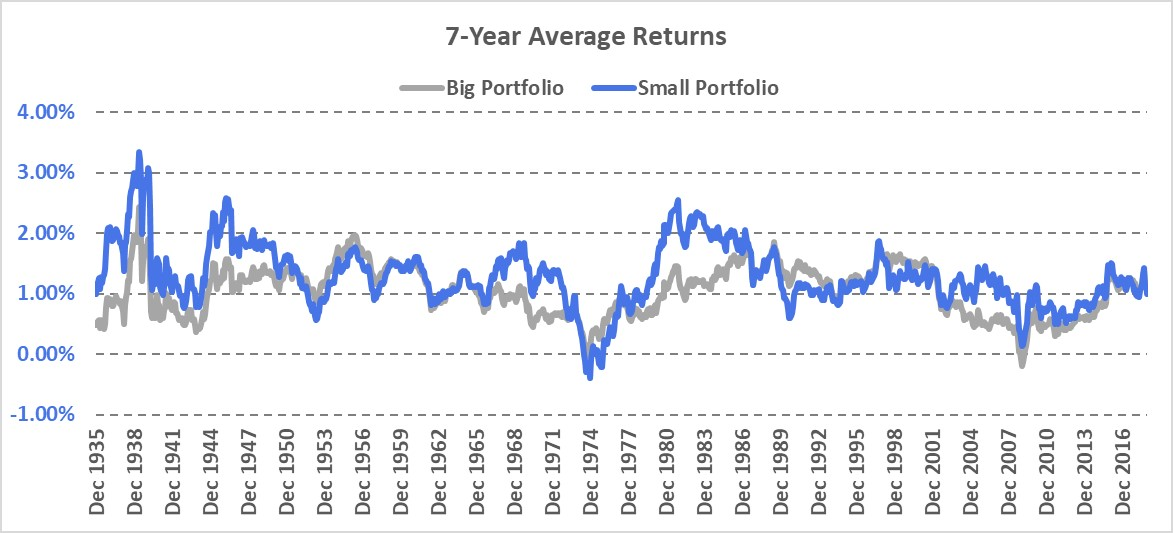
\includegraphics[width=0.9\linewidth]{SMB02}
	\caption*{Fig 02: Small Portfolio vs. Big Portfolio}
	\label{fig:label}
\end{figure}

\noindent Delving deeper, we found that the main driver behind the recent downtrend in rolling 7-year average SMB factor realisations stem mainly from rolling 7-year Big portfolio returns (grey line chart in Fig 02) seeing higher returns growth than rolling 7-year Small portfolio returns (blue line chart in Fig 01), thus gradually closing and even reversing the Small Minus Big (SMB) gap.  It remains to be seen when the long SMB play will be back in vogue, if ever. A summary of descriptive statistics of the SMB factor and our constructed SMB portfolio can be found below (see Table 07).

\newpage

\begin{figure}[h]
	\centering
	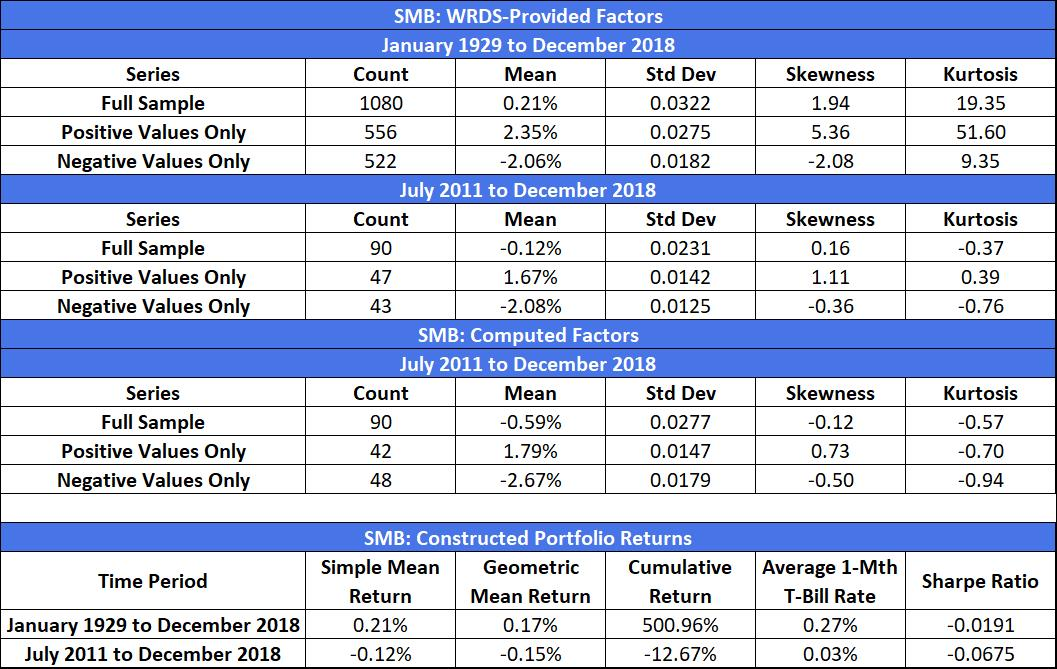
\includegraphics[width=0.8\linewidth]{SMB03}
	\caption*{Table 07: SMB Factor Summary Statistics}
	\label{fig:label}
\end{figure}

\noindent \textbf{The HML Factor}

\noindent Like the SMB factor, the HML factor was observed to exhibit mildly negative mean readings for the period between July 2011 and December 2018, though the HML factor's mean reading of -0.10\% is deemed to be statistically indifferent from 0 at the 5\% significance level. Further, the HML factor was seen to have displayed more consistently and persistently positive readings over the extended sample period of between January 1929 and December 2018 compared to the SMB factor.

\begin{figure}[h]
	\centering
	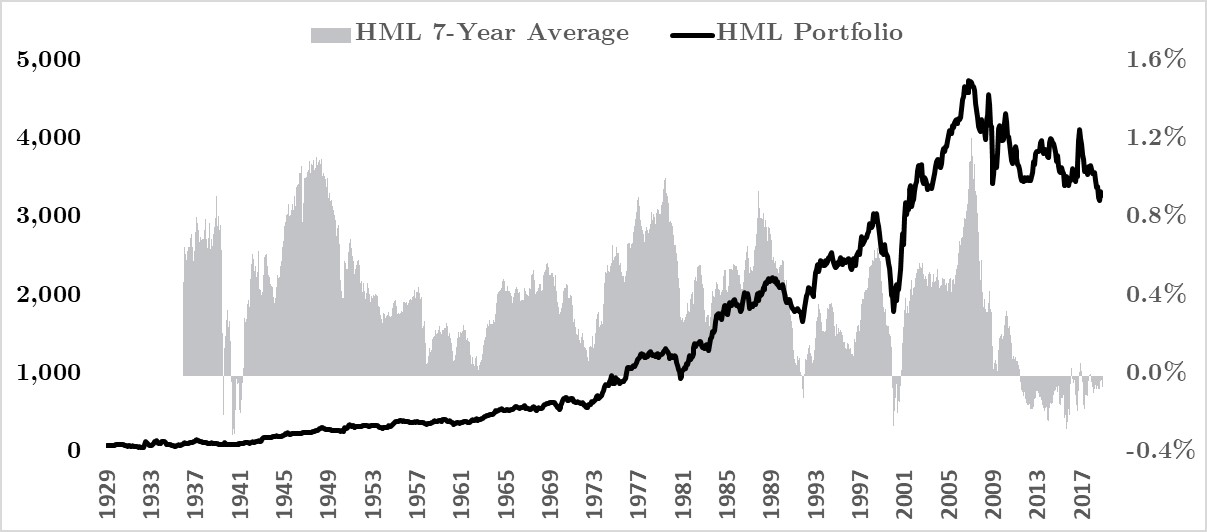
\includegraphics[width=0.9\linewidth]{HML01}
	\caption*{Fig 03: HML Portfolio \& Rolling 7-Year Average HML Returns}
	\label{fig:label}
\end{figure}

\noindent This inference can be drawn from lesser observed instances of negative rolling 7-year average HML factor readings (consistency) and longer streaks of positive rolling 7-year average HML factor readings (persistence) when compared to those of the SMB factor. This makes the unravelling of the HML factor's positive readings over the recent decade all the more an unprecedented one, which also explains the divergence between our observed mean HML and that of Fama and French (1993). 

\begin{figure}[h]
	\centering
	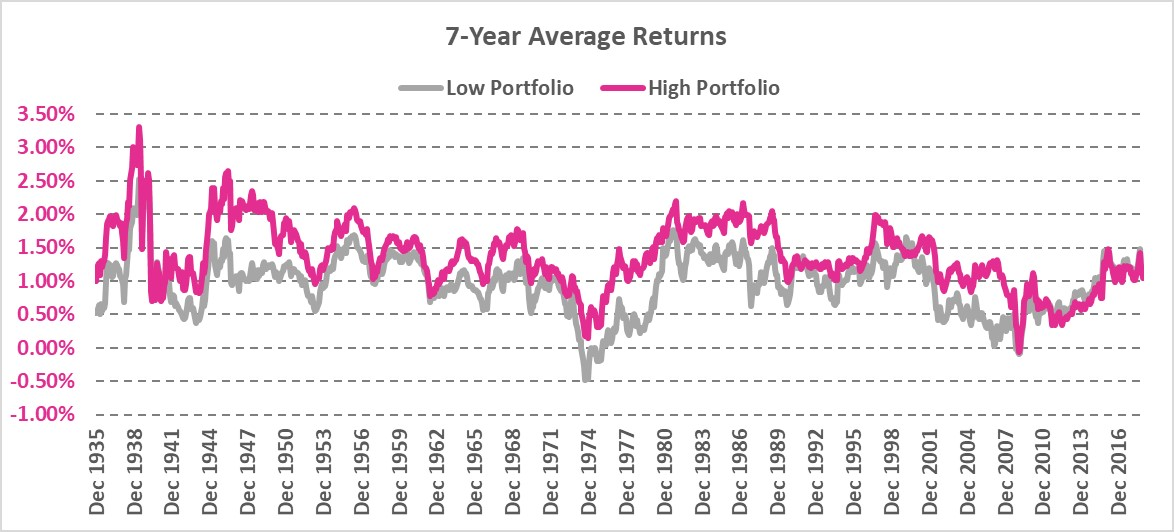
\includegraphics[width=0.9\linewidth]{HML02}
	\caption*{Fig 04: High Portfolio vs. Low Portfolio}
	\label{fig:label}
\end{figure}

\noindent It was also observed that our constructed HML portfolio has grossly outperformed our constructed SMB portfolio over the extended sample period in terms of nominal returns. The HML portfolio clocked 3,200.59\% returns while the SMB portfolio only clocked 500.96\%, with the latter's Sharpe ratio coming up as negative for returns over the extended sample period. With that said, both long SMB and long HML strategies have fallen short during our original sample period of between July 2011 to December 2018. A summary of descriptive statistics of the HML factor and our constructed HML portfolio can be found below (see Table 08).

\begin{figure}[h]
	\centering
	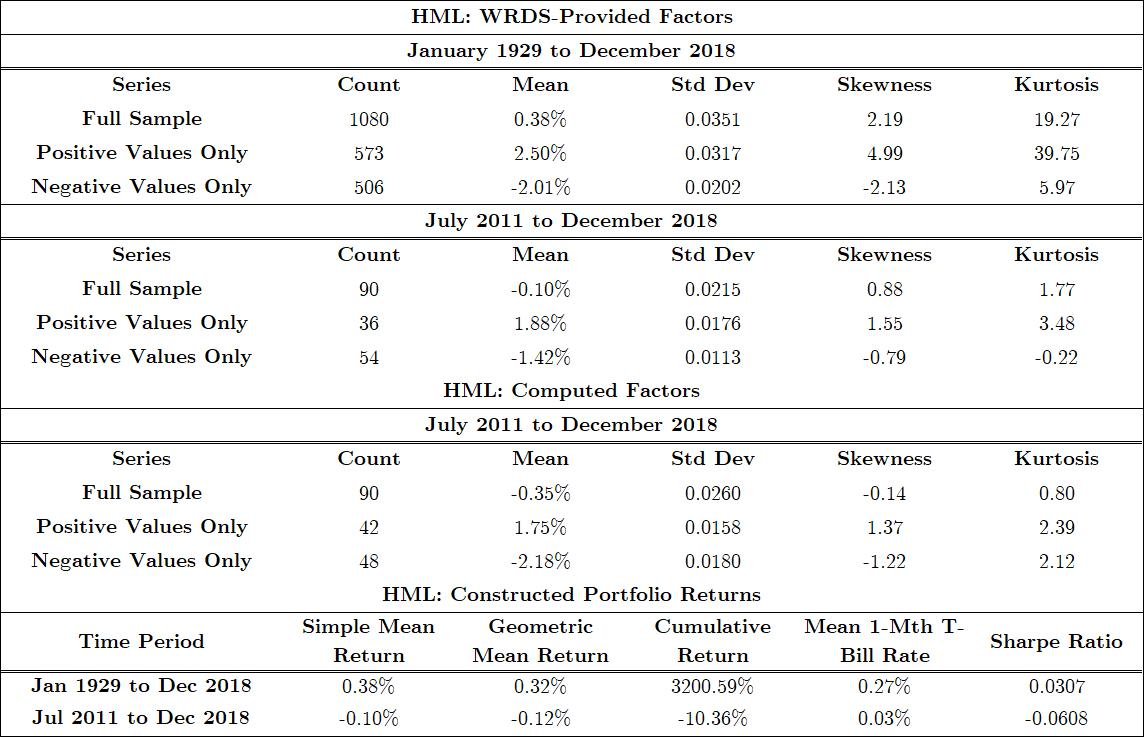
\includegraphics[width=0.8\linewidth]{HML03}
	\caption*{Table 08: HML Factor Summary Statistics}
	\label{fig:label}
\end{figure}

\newpage

\noindent \textbf{The UMD Factor}

\noindent We also looked at one of the additional stock market factors introduced and popularised by Carhart (1997): the momentum factor (UMD). As with the case of the SMB and HML factors, we constructed a UMD portfolio and the rolling 7-year average of UMD readings using data supplied by the WRDS and tracked their fluctuations over the extended sample period.

\begin{figure}[h]
	\centering
	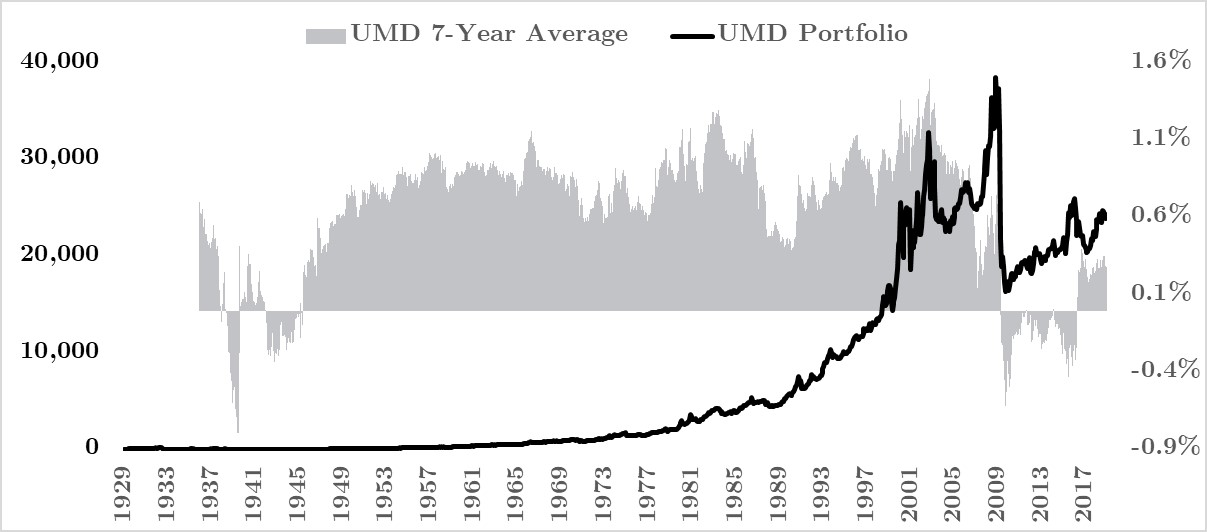
\includegraphics[width=0.9\linewidth]{UMD01}
	\caption*{Fig 05: UMD Portfolio \& Rolling 7-Year Average UMD Returns}
	\label{fig:label}
\end{figure}

\noindent Like the HML factor, it was observed that the UMD factor is consistently and persistently positive given the relatively high frequency of observed instances of positive rolling 7-year average UMD factor readings (consistency) and the long streaks of positive rolling 7-year average UMD factor readings (persistence). Also, like the SMB and HML factors, we observed an unravelling of the long UMD play in the recent decade, though said unravelling took place relatively earlier from April 2009 and has already recovered since April 2016. 

\begin{figure}[h]
	\centering
	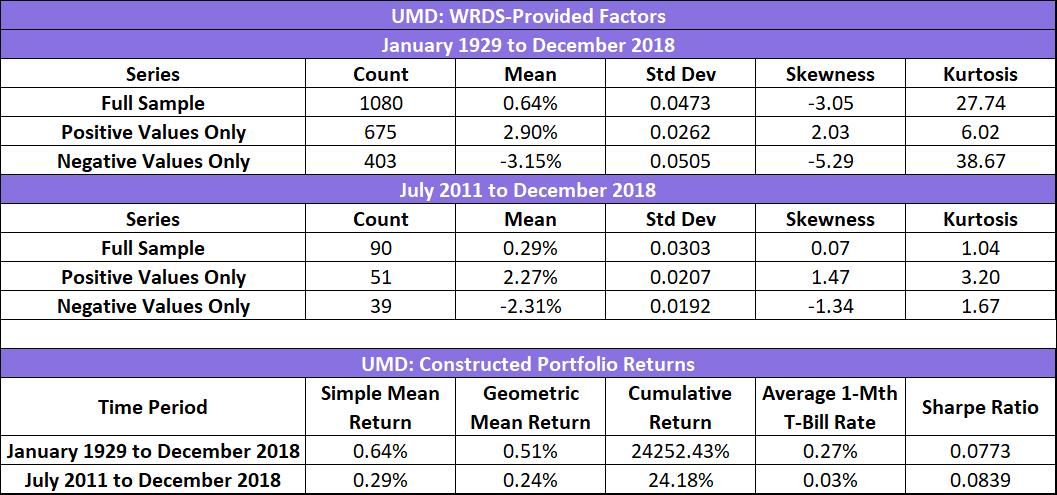
\includegraphics[width=0.8\linewidth]{UMD02}
	\caption*{Table 09: UMD Factor Summary Statistics}
	\label{fig:label}
\end{figure}

\noindent In terms of cumulative returns, the long UMD play has grossly outperformed both the long SMB play and the long HML play, with cumulative nominal returns of 24,252.43\% observed over the extended sample period and 24.18\% over the original sample period. On a risk-adjusted basis and in terms of Sharpe ratios, the long UMD outperforms the long SMB play and the long HML play too. A summary of descriptive statistics of the UMD factor and our constructed UMD portfolio can be found above (see Table 09).

\end{document}